\documentclass{beamer}
\usepackage{default}
\usepackage{amsmath}
\usepackage{graphicx}
\usepackage{adjustbox}  % Allows for fitting tables into slide
\usepackage{hyperref}
\usepackage{threeparttable}
\usepackage{caption}
%\usepackage{subcaption}
\usepackage{natbib}
\usepackage{adjustbox}
\usepackage{subcaption}
%\usetheme{AnnArbor}
%\usetheme{Antibes}
%\usetheme{Bergen}
%\usetheme{Berkeley}
%\usetheme{Berlin}
%\usetheme{Boadilla}
%\usetheme{boxes}
\usetheme{CambridgeUS}
%\usetheme{Copenhagen}
%\usetheme{Darmstadt}
%\usetheme{default}
%\usetheme{Frankfurt}
%\usetheme{Goettingen}
%\usetheme{Hannover}
%\usetheme{Ilmenau}
%\usetheme{JuanLesPins}
%\usetheme{Luebeck}
%\usetheme{Madrid}
%\usetheme{Malmoe}
%\usetheme{Marburg}
%\usetheme{Montpellier}
%\usetheme{PaloAlto}
%\usetheme{Pittsburgh}
%\usetheme{Rochester}
%\usetheme{Singapore}
%\usetheme{Szeged}
%\usetheme{Warsaw}

% colortheme to choose one 

%\usecolortheme{beaver}
%\usecolortheme{crane}
%\usecolortheme{default}
\usecolortheme{dolphin}
%\usecolortheme{seagull}
%\usecolortheme{seahorse}
%\usecolortheme{whale}


% fond theme to choose one 
%\usefonttheme{structuresmallcapsserif}
%\usefonttheme{structureitalicserif}
%\usefonttheme{structurebold}
\usefonttheme{serif}
%\usefonttheme{professionalfonts}
%\usefonttheme{default}

\title{Perceived Income Risks}


% A subtitle is optional and this may be deleted

\author{Tao Wang \\ Johns Hopkins University}
% - Give the names in the same order as the appear in the paper.
% - Use the \inst{?} command only if the authors have different
%   affiliation.

\date{\today}
% - Either use conference name or its abbreviation.
% - Not really informative to the audience, more for people (including
%   yourself) who are reading the slides online

% This is only inserted into the PDF information catalog. Can be left
% out. 

% If you have a file called "university-logo-filename.xxx", where xxx
% is a graphic format that can be processed by latex or pdflatex,
% resp., then you can add a logo as follows:

% \pgfdeclareimage[height=0.5cm]{university-logo}{university-logo-filename}
% \logo{\pgfuseimage{university-logo}}

% Delete this, if you do not want the table of contents to pop up at
% the beginning of each subsection:
\AtBeginSubsection[]
{
	\begin{frame}<beamer>{Outline}
	\tableofcontents[currentsection]
\end{frame}
}

\begin{document}
	

\begin{frame}
	\titlepage
\end{frame}
\begin{frame}{Outline}
	\tableofcontents
	% You might wish to add the option [pausesections]
\end{frame}


\section{Motivation}

\begin{frame}{Motivation}
	\begin{itemize}
		\item ddddddddd
	\end{itemize}
\end{frame}


\begin{frame}{This paper's agenda}
	\begin{enumerate}
		\item dddd
	\end{enumerate}
\end{frame}


\begin{frame}{Literature}
\begin{itemize}
	\item ddddd
	\begin{itemize}
		\item dddd
	\end{itemize}
\end{itemize}
\end{frame}

\section{Stylized facts}



\begin{frame}{Data}
\begin{table}
	\centering
	\caption{Survey of Consumer Expectations}
	\label{SCE_data_sum}
	\adjustbox{max height=0.5\textheight, max width=\textwidth}{ 
			\begin{tabular}{lll}
				\hline 
				Time period                                    & 2013M6-2018M6            \\
				Frequency                                      & monthly                                 \\
				Sample size                                    & 1,300                                  \\
				Density variable                    &  \textcolor{blue}{{1-yr-ahead earning growth   \\ (same position/hours)} }           \\
				Pannel structure                               & stay up to 12 months      \\
				Demographics                     & educ, income, age        \\
				\hline 
		\end{tabular}
	}
	\end{table}
	\begin{itemize}
		\item density estimation following (\citet{engelberg_comparing_2009})
		\item exclude top and bottom 5\% values for forecast errors and uncertainty
	\end{itemize}
\end{frame}

\begin{frame}{Definitions}
	\begin{itemize}
		\item Moments:
		\begin{itemize}
			\item expected growth, $\bar \Delta (y_i)$
			\item variance: $\bar \sigma^2_i(\Delta y_i)$
			\item skewness: $\bar {skew}_i(\Delta y_i)$
		\end{itemize}
		\item Both nominal and real (because the inflation density forecst is available)
		\begin{itemize}
			\item $\bar \sigma_i^2(\Delta y^r) =\bar \sigma_i^2(\Delta y^n) +  \sigma_i^2(\pi)$  
		\end{itemize}
		\item Can be adjusted with unemployment risk, therefore, the perceived risk of same job is just a lower bound for real income risk. 
	\end{itemize}
\end{frame}



\subsection{Cross-sectional distributions of subjective income risks}

\begin{frame}{Assuring evidence}
		\begin{figure}
		\centering
		\label{InfVar}
		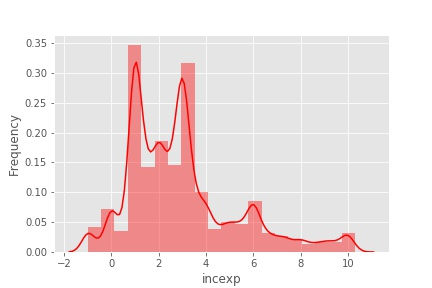
\includegraphics[width=0.4\textwidth]{figures/hist_incexp}
		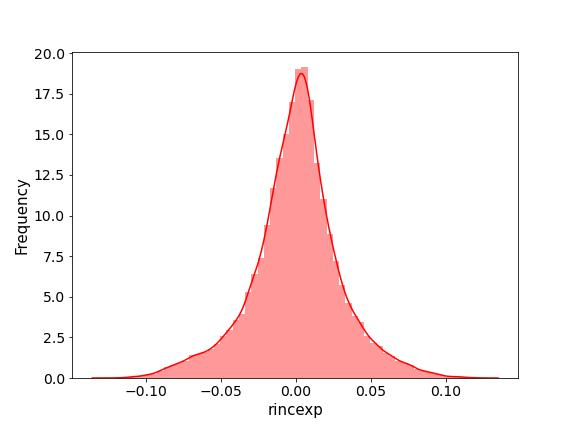
\includegraphics[width=0.4\textwidth]{figures/hist_rincexp.png} \\
		\vspace 
		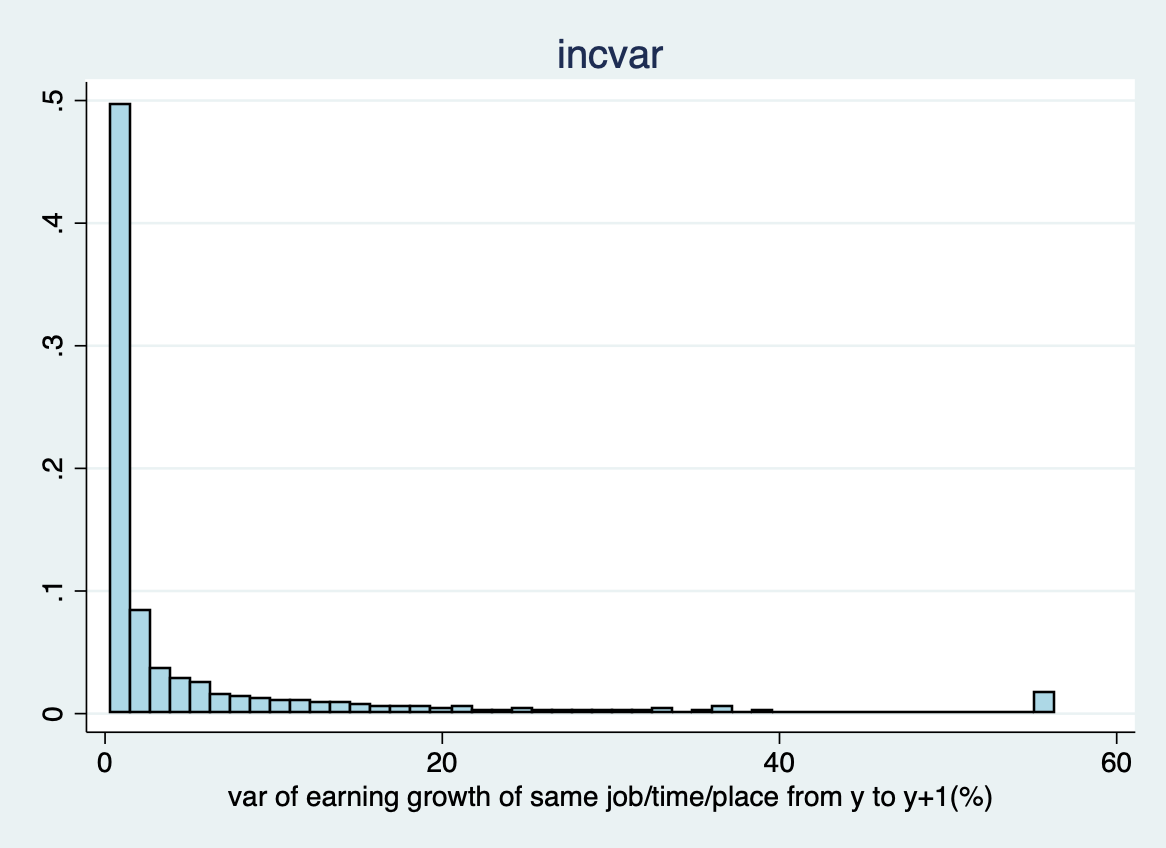
\includegraphics[width=0.4\textwidth]{figures/hist_incvar.png}
		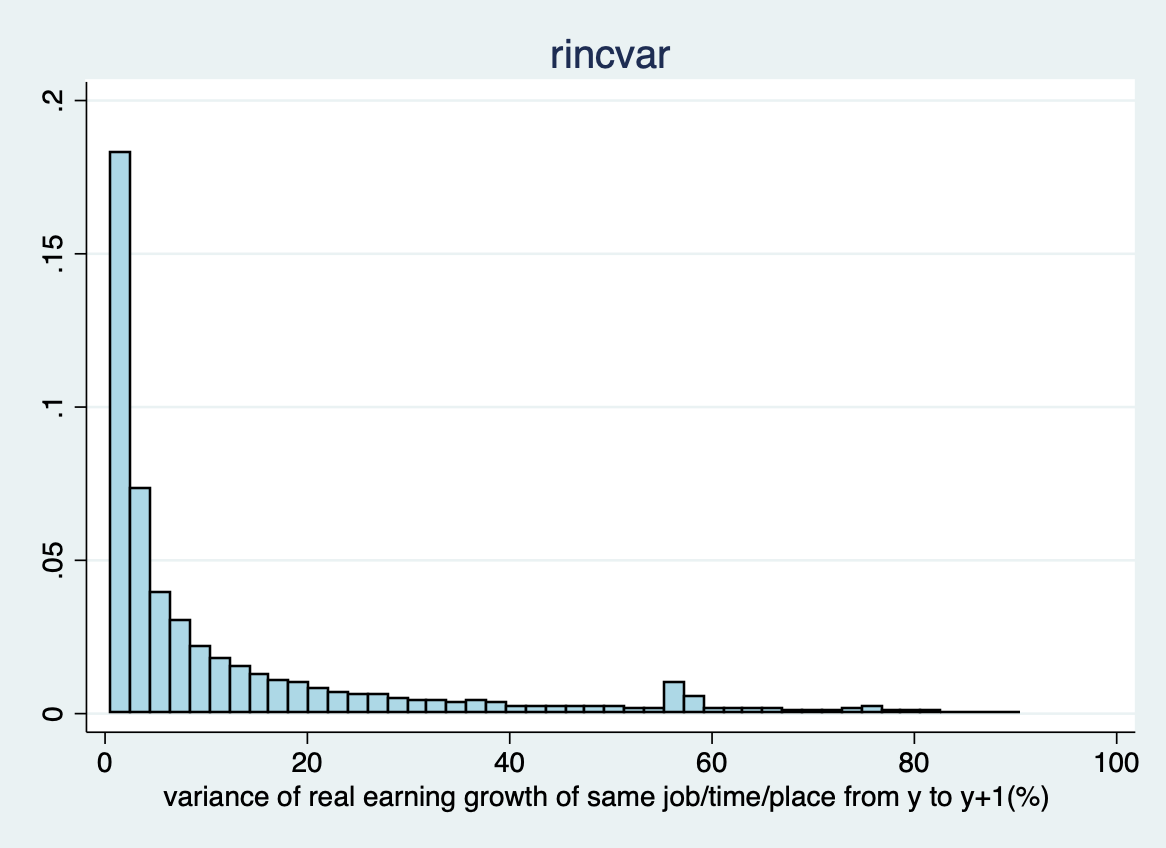
\includegraphics[width=0.4\textwidth]{figures/hist_rincvar.png}
	\end{figure}
	\begin{itemize}
		\item Nominal rigity can be seen from the expected norminal earning growth, while real expected growth become symmetric 
	\end{itemize}
\end{frame}


\begin{frame}{Assuring evidence}
	\begin{itemize}
		\item Nominal rigity seen from the expected earning growth
		\item Real growth become more symmetric 
	\end{itemize}
\end{frame}


\subsection{Correlation with stock market returns}

\subsection{Perceived risks and economic decisions}

\section{Model (work in progress)}

\begin{frame}{Model ingredients}

\begin{enumerate}
	\item imperfect understanding of the income process, a deviation from rational expectation benchmark. 
	\begin{itemize}
		\item experience-based learning 
	\end{itemize}
\item finite-period life cycle with a constant probability of death 
\item uninsured idiosyncratic risks and aggregate risks, workhorse assumption of the HANK literature
\item single asset, i.e. no distinction between liquid and iliquid assets 
\end{enumerate}
	
\end{frame}



\begin{frame}{Intuitions behind the model mechanisms}
	\begin{itemize}
		\item imperfect understanding $\rightarrow$ heterogeneous perception of risks $\plus$ uninsurance of risks $\rightarrow$ difference in precautionary motives and MPCs across populations $\rightarrow$ potential amplification of aggregate MPC. 
\end{itemize}
\end{frame}

%%%%%%%%%%%%%%%%%%%%%%%%%



\begin{frame}{Basic patterns: uncertainty and realized inflation}
	\begin{figure}
		\centering
		\label{InfVar}
		\includegraphics[width=0.3\textwidth]{figuresDraft/Inf1yf_CPIAU_varSPFCPIQ.png}
		\includegraphics[width=0.3\textwidth]{figuresDraft/Inf1yf_PCE_varSPFPCEQ.png}
		\includegraphics[width=0.3\textwidth]{figuresDraft/Inf1yf_CPIAU_varSCEM.png}
	\end{figure}
\end{frame}


\begin{frame}{Basic patterns: uncertainty and the size of forecast errors}
	\begin{figure}
		\centering
		\label{FEVar}
		\includegraphics[width=0.3\textwidth]{figuresDraft/SPFCPI_abFE_varSPFCPIQ.png}
		\includegraphics[width=0.3\textwidth]{figuresDraft/SPFPCE_abFE_varSPFPCEQ.png}
		\includegraphics[width=0.3\textwidth]{figuresDraft/SCE_abFE_varSCEM.png}
	\end{figure}
\begin{itemize}
\item no evidence for positive correlation betwen high ex ante uncertainty and ex post forecast errors.
\end{itemize}
\end{frame}



%%%%%%%%%%%%%%%%%%%

\begin{frame}{Some Table Results}
	\begin{table}
		\centering
		\caption{SMM Estimates of SE: professionals}
		\label{SMM_Est_SE_SPF_Table}
		\adjustbox{max height=0.5\textheight, max width=\textwidth}{ 

	}
	\end{table}
	\begin{itemize}
		\item $\lambda$: update rate in SE
	\end{itemize}
\end{frame}



\begin{frame}{Some Figures}
	\begin{figure}[ht]
		\label{figurelabel}
		\begin{subfigure}[b]{0.2\textwidth}
			\centering
			\caption{FE}
			\includegraphics[width=\textwidth, height = 0.8\textheight]{figuresDraft/spf_se_est_diag0.png}
		\end{subfigure}
		\hfill
		\begin{subfigure}[b]{0.2\textwidth}
			\caption{Disg}
			\includegraphics[width=\textwidth, height = 0.8\textheight]{figuresDraft/spf_se_est_diag1.png}
		\end{subfigure}
		\hfill
		\begin{subfigure}[b]{0.2\textwidth}
			\caption{FE/Disg}
			\includegraphics[width=\textwidth, height = 0.8\textheight]{figuresDraft/spf_se_est_diag2.png}
		\end{subfigure}
	\end{figure}
\end{frame}


%%%%%%%%%%%%%%%%%%%%%%%%%%%%%%%%%



\section{Conclusion}

\begin{frame}{Conclusion}
	\begin{itemize}
		\item ddddd
	\end{itemize}	
\end{frame}

\section*{Appendix}

\begin{frame}[Density estimation and robustness of my results]
	\begin{itemize}
		\item ddd
	\end{itemize}
\end{frame}

\bibliographystyle{apalike}
\bibliography{PerceivedIncomeRisk}


\end{document}
